\section*{Теория}

\subsection*{Уравнение колебательного контура}

При рассмотрении физических процессов в электрических цепях используются следующие предположения. Во-первых, все элементы электрической цепи считаются \textit{идеальными}. Предполагается, что у катушек индуктивности и конденсаторов нет омического сопротивления, источник напряжения обладает нулевым сопротивлением, а источник тока бесконечно большим, и т.д. Такое представление упрощает анализ физических процессов в электрических цепях. Если же такие предположения вносят большую погрешность, то в схему добавляются дополнительные идеальные элементы, которые учитывают особенности физических процессов в конкретных случаях. 

Во-вторых, рассматриваются \textit{квазистационарные процессы}. Известно, что электромагнитные колебания распространяются с конечной скоростью. В данной работе рассматриваются такие электрические цепи, в которых время установления электромагнитных колебаний пренебрежимо мало. 

\begin{wrapfigure}{left}{0.22\textwidth}
	\vspace{-10pt}
	\centering
	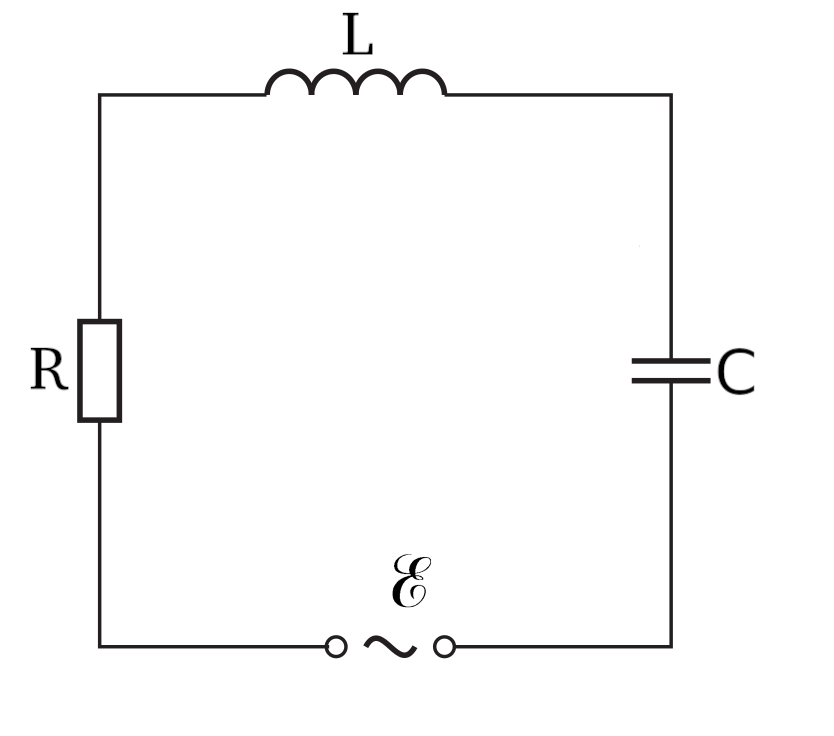
\includegraphics[width=0.2\textwidth]{../res/seq_osc_circ.png}
	\caption{Последовательный колебательный контур}
	\label{fig:seq_osc_circ}
\end{wrapfigure}

Рассмотрим последовательный колебательный контур без источника ЭДС (рис. $\ref{fig:seq_osc_circ}$).  Пусть напряжение на конденсаторе меняется по закону $U = U(t)$. Тогда, согласно второму правилу Кирхгофа, сумма падений напряжений равна 0:
$$
L \frac{dI}{dt} + U + RI = 0
$$
Ток через конденсатор определяется из соотношения
$$
I = \frac{dq}{dt} = C\frac{dU}{dt}
$$
Тогда получим дифференциальное уравнения второго порядка, описывающее \textit{свободные колебания} в линейной системе:
$$
LC \frac{d^2 U}{dt^2} + RC \frac{dU}{dt} + U = 0
$$
Данное уравнение можно переписать в виде:
\begin{equation*}
	\ddot{U} + 2\gamma \dot{U} + \omega_0^2 U = 0
	\label{eq:diff_eq}
\end{equation*}
где введены обозначения $\gamma = \frac{R}{2L}$ -- \textit{коэффициент затухания}, $\omega_0 = \frac{2\pi}{T_0} = \frac{1}{\sqrt{LC}}$ -- \textit{собственная частота} колебательной системы, $T_0 = 2\pi \sqrt{LC}$ -- \textit{период собственных колебаний}.

Найдём решение однородного дифференциального уравнения с постоянными коэффициентами. Запишем характеристическое уравнение:
$$
\lambda^2 + 2\gamma \lambda + \omega_0^2 = 0
$$
$$
D_1 = \frac{D}{4} = \gamma^2 - \omega_0^2
$$
В зависимости от знака дискриминанта квадратного уравнения возможны три случая.

\begin{enumerate}
	\item \textit{Затухающие колебания}.
	
	Рассмотрим случай, когда $D_1 < 0$. Тогда $0 < \gamma < \omega_0$, что эквивалентно
	$$
	0 < R < 2 \sqrt{\frac{L}{C}} = R_{кр}
	$$
	Сопротивление $R_{кр} = 2 \sqrt{\frac{L}{C}}$ называется критическим, а $\rho = \sqrt{\frac{L}{C}}$ -- волновым.
	
	В рассматриваемом случае характеристическое уравнение имеет два комплексных корня 
	$$
	\lambda_{1,2} = -\gamma \pm j\sqrt{\omega_0^2 - \gamma^2}
	$$
	Величину $\omega = \sqrt{\omega_0^2 - \gamma^2}$ называют частотой свободных колебаний. Решением уравнения будет
	$$
	U(t) = U_1 \cdot e^{-\gamma t} \cdot e^{-j\omega t} + U_2 \cdot e^{-\gamma t} \cdot e^{j\omega t}
	$$
	где $U_1$ и $U_2$ -- произвольные постоянные.
	
	Полученное уравнение можно представить в виде
	\begin{equation*}
		U(t) = U_0 e^{-\gamma t} sin(\omega t + \varphi_0)
		\label{eq:damp_osc}
	\end{equation*}
	Данное уравнение является гармоническим с фазой $\omega t + \varphi_0$ и экспоненциально убывающей амплитудой $U_0 e^{-\gamma t}$.
	
	График зависимости напряжения от времени представлен на рисунке $\ref{fig:damp_osc}$.
	
	\begin{figure}[H]
		\vspace{-10pt}
		\centering
		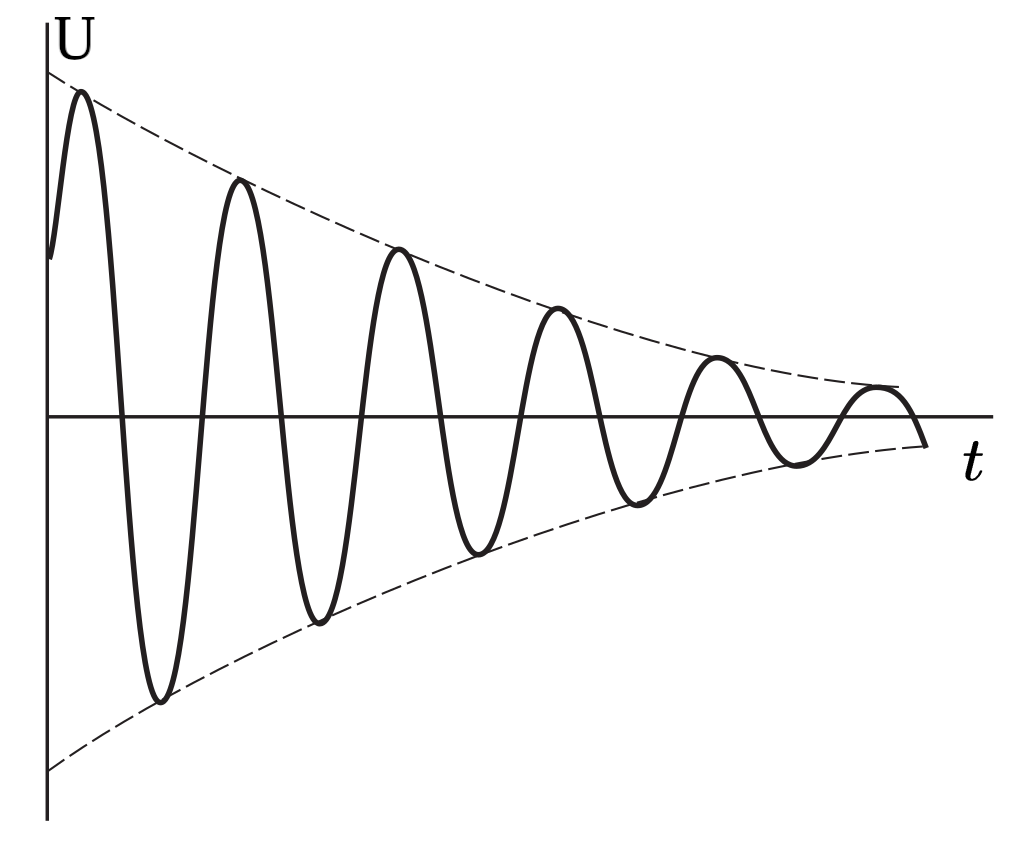
\includegraphics[width=0.3\textwidth]{../res/damp_osc.png}
		\caption{Затухающие колебания}
		\label{fig:damp_osc}
	\end{figure}

	С точки зрения математики данный колебательный процесс не периодичен. Тем не менее функция $U(t)$ обращается в ноль или достигает экстремумов через один и тот же промежуток времени, который называю \textit{периодом затухающих колебаний}.
	
	\item \textit{Критический режим}. 
	
	Рассмотрим случай, когда $D_1 = 0$. Тогда 
	$$
	\gamma = \omega_0
	$$
	Характеристическое уравнение имеет один корень
	$$
	\lambda = - \gamma
	$$
	Решением исходного уравнения будет
	$$
	U(t) = U_0 e^{-\gamma t}
	$$
	где $U_0$ -- постоянная, определяемая из начальных условий.
	
	Заметим, что данный режим физически не реализуем, так как равенство $\gamma = \omega_0$ не может быть выполнено точно. Данный случай нужно рассматривать как переходный между затухающими колебаниями и апериодическим режимом.
	
	\item \textit{Апериодический режим}. 
	
	Рассмотрим случай, когда $D_1 > 0$. Тогда $0 < \omega_0 < \gamma$. Характеристическое уравнение имеет два действительных корня
	$$
	\lambda_{1,2} = -\gamma \pm \sqrt{\omega_0^2 - \gamma^2}
	$$
	Решением дифференциального уравнения будет
	$$
	U(t) = e^{-\gamma t} \cdot (U_1 e^{-j\omega t} + U_2 e^{j\omega t})
	$$
	где $U_1$ и $U_2$ -- произвольные постоянные.
\end{enumerate}

\subsection*{Характеристики затухающих колебаний}

Важными характеристиками колебательных систем являются добротность $Q$ и логарифмический декремент $d$.

Логарифм отношения амплитуд колебаний в двух последовательных максимумах называется логарифмическим декрементом
$$
d = \ln{\left(\frac{A_n}{A_{n+1}}\right)}
$$
Определив положения последовательных максимумов из формулы $\ref{eq:damp_osc}$, можно получить следующее соотношение
\begin{equation*}
	d = \gamma T
	\label{eq:log_dec}
\end{equation*}
где $T$ -- период затухающих колебаний.

\textit{Постоянной времени затухания} $\tau$ называется время, за которое амплитуда колебаний убывает в $e$ раз. Коэффициент затухания и постоянная времени связаны соотношением
\begin{equation*}
	\tau = \frac{1}{\gamma}
	\label{eq:const_time}
\end{equation*}

Из уравнений $\ref{eq:log_dec}$ и $\ref{eq:const_time}$ следует, что логарифмический декремент можно определить как число полных колебаний $N = \frac{\tau}{T}$ за время затухания $\tau$:
$$
d = \frac{1}{N}
$$

Добротностью колебательной системы $Q$ называется
$$
Q \equiv \frac{\pi}{d} = \frac{\pi}{\gamma T} = \frac{\omega}{2 \gamma}
$$ 
Чем выше добротность колебательной системы, тем меньше будут потери энергии. Докажем данное утверждение.

Амплитуда колебаний напряжение за период уменьшается в $e^{\gamma T}$ раз. Полная энергия системы $W$ определяется как максимальная энергия электрического поля конденсатора или магнитного поля индуктивности
$$
W = \frac{CU^2}{2} = \frac{LI^2}{2}
$$
Из этого соотношения видно, что за период энергия системы уменьшается как квадрат амплитуды в $e^{2\gamma T}$ раз.
Тогда потери энергии системы равно
$$
\Delta W = W(t_0) - W(t_0 + T) = (1 - e^{-2\gamma T}) W(t_0)
$$
Если затухание мало, то есть $\gamma T \ll 1 \Rightarrow Q \gg 1$, то экспоненту можно разложить по формуле Тейлора
$$
\Delta W \approx 2 \gamma T W
$$
$$
\frac{W}{\Delta W} = \frac{1}{2\gamma T} = \frac{1}{2\pi}Q
$$
Таким образом, добротность с энергетической точки зрения определяет отношении энергии системы к потерям за период.

\subsection*{Вынужденные колебания}

Если в цепь последовательного колебательного контура включен гармонический источник ЭДС $\varepsilon(t) = \varepsilon_0 \cos{(\omega t)}$, то
$$
\ddot{U} + 2\gamma \dot{U} + \omega_0^2 U = \frac{\varepsilon_0}{LC} \cos{(\omega t)}
$$
Решением неоднородного дифференциального уравнения будет сумма однородного и частного решений
$$
U_{общ}(t) = U_{одн}(t) + U_{част}(t)
$$
Решением однородного уравнения будут затухающие колебания
$$
U_{одн}(t) = U_0 e^{-\gamma t} sin(\omega t + \varphi_0)
$$
Частное решение неоднородного уравнения будем искать в виде:
$$
U_{част}(t) = A e^{j \omega t}
$$
Неоднородность уравнения в комплексной форме равна
$$
\varepsilon = \frac{\varepsilon_0}{LC}e^{j \omega t}
$$
Подставив частное решение в исходное уравнение находим
$$
U_{част}(t) = \frac{\varepsilon_0 e^{j \omega t}}{LC (\omega_0^2 + 2 j \gamma \omega  - \omega^2)}
$$
Решением является только действительная часть, тогда
$$
U_{част}(t) = \frac{\varepsilon_0}{LC} \frac{1}{\sqrt{(\omega_0^2 - \omega^2)^2 + 4 \omega^2 \gamma^2 }} \cos{\left(\omega t - \arctg{\frac{2 \omega \gamma}{\omega_0^2 - \omega^2}}\right)}
$$
Итого уравнением вынужденных колебаний будет
$$
U(t) = U_0 e^{-\gamma t} sin(\omega t + \varphi_0) +  \frac{\varepsilon_0}{LC} \frac{1}{\sqrt{(\omega_0^2 - \omega^2)^2 + 4 \omega^2 \gamma^2 }} \cos{\left(\omega t - \arctg{\frac{2 \omega \gamma}{\omega_0^2 - \omega^2}}\right)}
$$
Заметим, что амплитуда однородного решения убывает экспоненциально, а амплитуда частного решения остается постоянной. Поэтому, через большой промежуток времени, напряжение будет изменяться по закону $U(t) \approx U_{част}(t)$. Итого, установившимися вынужденными колебаниями будут гармонические колебания с частотой вынуждающей ЭДС.

\subsection*{Резонанс в последовательном колебательном контуре}

Рассмотрим последовательный колебательный контур. Пусть к нему подключен идеальный источник ЭДС, обладающий бесконечно малым внутренним сопротивлением, задающий во внешней цепи напряжение, изменяющееся по гармоническому закону $\varepsilon = \varepsilon_0 \cos{\left(\omega t + \phi_0\right)}$.

\begin{figure}[H]
	\vspace{-10pt}
	\centering
	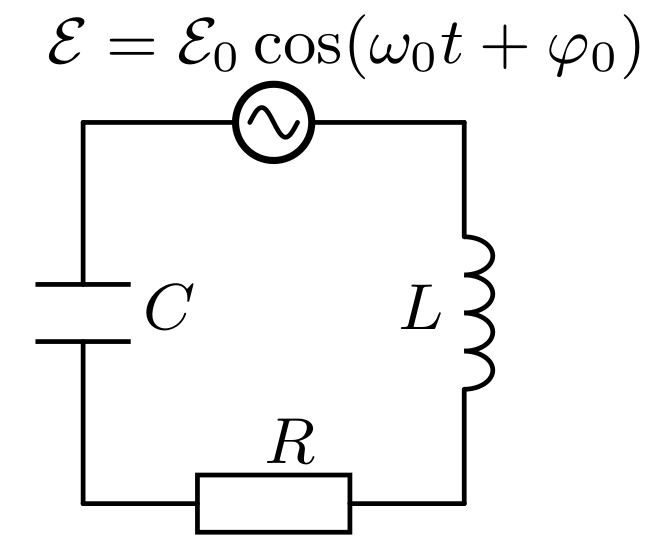
\includegraphics[width=0.4\textwidth]{../res/seq_contour.png}
	\caption{Последовательный колебательный контур}
	\label{fig:seq_contour}
\end{figure}

Методом комплексных амплитуд определим зависимости напряжения и тока на элементах цепи:
\begin{equation*}
	\begin{split}
		U_C &= \varepsilon_0 \frac{\rho}{Z_0} \frac{\omega_0}{\omega} \cos \left(\omega t - \varphi_C\right) \\
		U_L &= \varepsilon_0 \frac{\rho}{Z_0} \frac{\omega}{\omega_0} \cos \left(\omega t - \varphi_L\right) \\
		I &= \frac{\varepsilon_0}{Z_0} \cos \left(\omega t - \varphi_I\right) \\
		Z_0 &= R \sqrt{1 + \left[\frac{\rho}{R} \left(\frac{\omega}{\omega_0} - \frac{\omega_0}{\omega}\right)\right]^2} \\
		\varphi_I &= \arctg{\left[\frac{\rho}{R} (\frac{\omega}{\omega_0} - \frac{\omega_0}{\omega})\right]} \\
		\varphi_C &= \varphi_I + \frac{\pi}{2} \\
		\varphi_L &= \varphi_I - \frac{\pi}{2}
	\end{split}
\end{equation*}

Далее будем рассматривать высокодобротный колебательный контур вблизи резонансной частоты $Q \approx \frac{\rho}{R} \gg 1$. Тогда полученные уравнения можно упростить:
\begin{equation*}
	\begin{split}
		U_C &= \frac{Q \varepsilon_0 \omega_0}{\omega \sqrt{1 + (\tau \Delta \omega)^2}} \cos \left(\omega t - \varphi_C\right) \\
		U_L &= \frac{Q \varepsilon_0 \omega}{\omega_0 \sqrt{1 + (\tau \Delta \omega)^2}} \cos \left(\omega t - \varphi_L\right) \\
		I &= \frac{\varepsilon_0}{R \sqrt{1 + (\tau \Delta \omega)^2}} \cos \left(\omega t - \varphi_I\right) \\
		Z_0 &= R \sqrt{1 + (\tau \Delta \omega)^2} \\
		\varphi_I &= \arctg{\tau \Delta \omega}	
	\end{split}
\end{equation*}

При резонансе $\omega = \omega_0$, $\Delta \omega = 0$ и формулы можно упростить:
\begin{equation*}
	\begin{split}
		I &= \frac{\varepsilon_0}{R} \cos \left( \omega_0 t - \varphi_I \right) \\
		U_L &= Q \varepsilon_0 \cos \left( \omega_0 t - \varphi_L \right) \\
		U_C &= Q \varepsilon_0 \cos \left( \omega_0 t - \varphi_C \right) \\		
		\varphi_I &= 0 \\
		\varphi_C &= \frac{\pi}{2} \\
		\varphi_L &= -\frac{\pi}{2} \\
	\end{split}
\end{equation*}

Из полученных соотношений следует, что напряжение на конденсаторе $U_C$ отстает от внешнего тока по фазе на $\frac{\pi}{2}$. Напряжение на индуктивности опережает внешний ток по фазе на $\frac{\pi}{2}$.

Напряжение на конденсаторе и индуктивности в $Q$ раз больше внешнего напряжения. Поэтому резонанс в последовательном колебательном контуре называют \textit{резонансном напряжений}.
